%  Prerequisites
\chapter{State of the Art}
This chapter provides an overview of the concepts and technologies which are important in the field of my current work. First in Section \ref{lab:background} we define domain-specific terms. In Section \ref{lab:relWork} we discuss related work in the field.
In Section \ref{lab:systems}, we describe the systems, which will be used for this thesis.

\section{Background} \label{lab:background}

\subsection{Social Bots and Chatbots}
Bots in general are an interfaces, which provide automated services to end-users. In contrast to normal computer programs, bots use the services, which were designed for human users, such as browsing webpages and issuing API calls. Bots, which are deployed in social media, are called social bots. The definition of a social bot is provided by \cite{FVD*16b}:
\begin{quote}
	``A social bot is a computer algorithm that automatically produces content and interacts with humans on social media, [...]''
\end{quote}

Social bots are getting more and more popular in Human-Computer Interactin (HCI), by integrating automation into daily lives of people \cite{BFPN17}. Users can interact with a social bot through a dedicated channel, such as the chat functionality of a social network. Social bots, which use chats to interact with users are called chatbots, or conversational bots \cite{WWX*16}. Chatbots have recently become very popular in the context of customer care \cite{CHW*17,FVD*16b}, where they act as virtual assistants, which can answer simple questions \cite{CaWh14} or perform predefined tasks. They thereby assist companies in customer service as they are more economical and the staff can concentrate on less mundane tasks.

Chatbots can be classified into chit-chat chatbots, or task-oriented bots. A chit-chat bot engages users into interesting conversations.

We can distinguish between retrieval based chatbots and generic chatbots \cite{NLKl19,WWX*16}. Retrieval based bots are focussed on getting specific tasks done and focus less on engaging in a coherent conversation.

Retrieval based chatbots measure the similarity of user queries to candidate responses and run the task that is defined for the candidate repsonse. They do this by using natural language processing and machine learning techniques. Generic chatbots on the other hand also use machine-learning techniques to generate generic responses. An advantage of the generic chatbots is that they provide a better user experience as users can interact more naturally with them than with retrieval based chatbots.

Chatbots provide a better user experience \cite{CHW*17}, because the user is not required to memorize commands in order to get the desired results. This means that even non-trained users can use such chatbots. From such a standpoint, it becomes clear why such chatbots are desirable as assistants.

\subsection{Natural Language Understanding}
Natural Language Understanding (NLU) is a branch of Artificial Intelligence (AI), which tries to make computer programs understand the semantics of human language. It does this by transforming a block of input text into a data structure that is programmer-friendly but still describes the original meaning of the text \cite{CWB*11}.

Most NLU algorithms these days only look at the syntacticts of words, which relies on statistical features, such as word occurence frequency \cite{CaWh14}. However humans take far more information into consideration, as the reading of a word triggers a whole bunch of related concepts and experiences which are combined to give the understanding of a text.

Computers try to close this knowledge gap with computational models, which emulate human cognitive processing. By evaluating the results of those models for a given input, researchers can incrementally improve the accuracy of the model \cite{CaWh14}

\subsection{Machine Learning}
Machine learning is a branch of Artifial Intelligence, that specialises in systems that learn from past experience. Machine-learning algorithms can be subdivided into supervised and unsupervised learning \cite{MiBu16}.

Supervised machine-learning systems classify data based on a model that was previously trained on a labelled dataset. Such a dataset, which is also commonly called a trainingset, consists of pairs of input data and desired output data. The provided trainingset highgly influences the accuracy of the classifier. The higher, the qualitity, diversity and quantity of the trainingset, the better the resulting model will be able to classify intentions.

In contrast, unsupervised machine-learning techniques do not need a trainingset, but only rely on the input data to do the classification.
They are thereby able to be deployed in unknown complex environments \cite{Adam17}

Once a classifier is trained, it can be used by the chatbot to determine the intentions in chat and thereby run specific tasks that match those intentions.
Decision tree, Random-forest , neural networks are only a few examples of classifiers. Another prominent example for such a classifier are deep learing technologies, which are publicly available \cite{NLKl19}.

\subsection{Communities of Practice}
Communities of Practice (CoP) are groups of entities, which share a common research domain. The advantage of CoPs is that they enhance learning and transferring knowledge \cite{AMMi15}. In contrast to traditional knowledge systems, the transfer of knowledge is a social process, where an individual volontarily shares knowledge in the community.

\subsection{Measurement of Success}
In order to justify their existence, communities have to constantly be aware of their successes and failures. They need to constantly adjust measurements of success to satisfy current needs. Therefore a measurement of success is needed. Success criteria can be internal aspects, like project duration, cost and qualitity, as well as external aspects, like customer satisfaction \cite{AgRa06}.

In order to estimate success, a model is required. It is important to note, that a project can be evaluated from different perspectives, e.g. the developers, the customers or the end-users. In each of these perspectives, each dimension of success can be more, or less, important.
DeLone and McLean \cite{DeMc92} base their model on six different interdependant measures:
\begin{itemize}
	\item System Qualitity: metrics that describe the technical specifations of the system
	\item Information Quality: metrics about content qualitity
	\item Use: Metrics about how a system is used
	\item User Satisfaction: includes metrics which measure user experience
	\item Individual Impact: metrics about how a user adapts to the system
	\item Organizational Impact: metrics about how the system influences the community
\end{itemize}
\begin{figure}[!h]
	\centering
	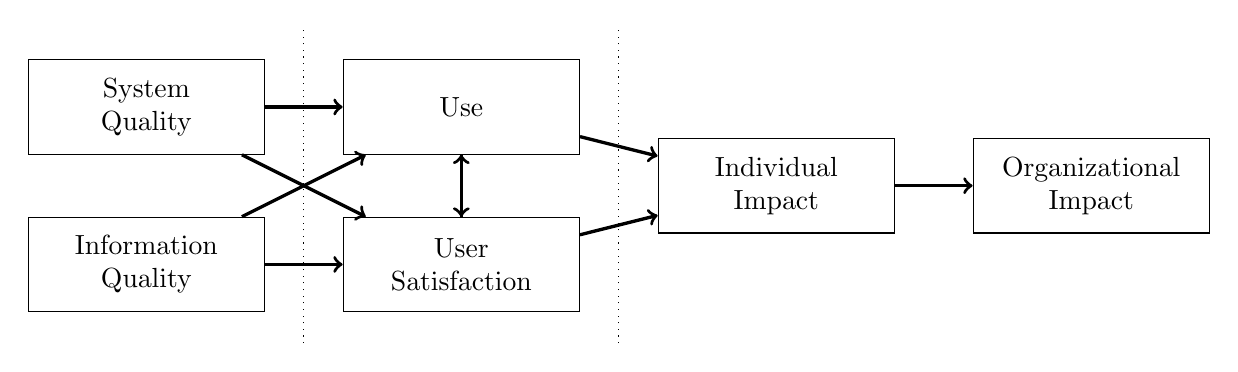
\begin{tikzpicture}[node distance=3.0cm and 6.0cm]
		\node[draw, align=center, minimum width=3cm, minimum height=1.2cm] at (0,2) (SysQ) {System\\ Quality};
		\node[draw, align=center, minimum width=3cm, minimum height=1.2cm] at (0,0) (InfoQ) {Information\\ Quality};
		\node[draw, align=center, minimum width=3cm, minimum height=1.2cm] at (4,2) (Use) {Use};
		\node[draw, align=center, minimum width=3cm, minimum height=1.2cm] at (4,0) (UserSat) {User\\ Satisfaction};
		\node[draw, align=center, minimum width=3cm, minimum height=1.2cm] at (8,1) (Indivi) {Individual\\ Impact};
		\node[draw, align=center, minimum width=3cm, minimum height=1.2cm] at (12,1) (Orga) {Organizational\\ Impact};
		\draw [->, very thick] (InfoQ) -- (Use);
		\draw [->, very thick] (InfoQ) -- (UserSat);
		\draw [->, very thick] (SysQ) -- (Use);
		\draw [->, very thick] (SysQ) -- (UserSat);
		\draw [->, very thick] (Use) -- (Indivi);
		\draw [->, very thick] (UserSat) -- (Indivi);
		\draw [->, very thick] (Use) -- (UserSat);
		\draw [->, very thick] (UserSat) -- (Use);
		\draw [->, very thick] (Indivi) -- (Orga);
		\draw[dotted] (2,-1) -- (2,3);
		\draw[dotted] (6,-1) -- (6,3);
	\end{tikzpicture}
	\caption{Community Information Systems Success Model by DeLone and McLean~\cite{DeMc92}}
	\label{CISModel}
\end{figure}

\subsection{Mediabase}
Mediabase is a database schema, which has been proposed to store Web 2.0 data in a dynamic way. Mediabase use graphs to model generated data. The nodes in those graphs are called \emph{Actors} and represent either a \emph{ Medium}, an \emph {Artifact}, a \emph{Member}, or a \emph{Network}. Furthermore, Mediabase includes \emph{Services} \cite{KlPe08}.
\begin{figure}
	\centering
	\includegraphics*[width=12cm]{related_work/mediabase.png}
\end{figure}


\subsection{GraphQL}
GraphQL\footnotemark is a query language specifation for web APIs. Instead of hitting multiple endpoints for different requests, users can query all data from one endpoint, by specfifying the kind of data that they need. Data objects are defined as a \emph{type}. GraphQL provides simple base-types like Int Float, Boolean and String.
\begin{lstlisting}[caption={Example of a GraphQL schema},captionpos=b]
    
type User {
  id: ID
  name: String
}
\end{lstlisting}


\footnotetext{GraphQL: \href{https://graphql.github.io/}{https://graphql.github.io/}}
\section{Related Work} \label{lab:relWork}

Creating a chatbot from scratch is a difficult challenge. Luckily, there are already publicly available frameworks, which can be used to create a variety of bots.

\subsection{Microsoft Bot Framework}
The Microsoft Bot Framework provides both an SDK\footnote{Azure Bot Service: \href{https://docs.microsoft.com/en-us/azure/bot-service/index-bf-sdk?view=azure-bot-service-4.0}{https://docs.microsoft.com/en-us/azure/bot-service/index-bf-sdk?view=azure-bot-service-4.0}}, as well as a GUI\footnote{Bot Framework Composer: \href{https://docs.microsoft.com/en-us/composer/}{https://docs.microsoft.com/en-us/composer/}} to create chatbots. Such bots use Language Understanding \footnote{Language Understanding: \href{https://www.luis.ai/}{https://www.luis.ai/}} to understand human requests. The Microsoft Bot Framework allows for an easy creation of a chatbot that can perform simple tasks, such as fetching weather reports, or answering FAQ questions \cite{CaWh14}. They can be deployed in a .NET or Node.js environment and can connect to a variety of different channels, such as Microsoft Teams, Amazon Alexa and Slack.

\subsection{RASA}
Rasa is an open sourced framework for building chat- and voice-based bots. The goal of RASA is to bring current advances in machine-learning to end-users, such that they can create chatbots in a simple way \cite{BFPN17}. The RASA system is split into a component for natural language understanding (RASA NLU) and a dialogue management component (RASA Core).

RASA NLU is used to extract the intents of a user message with a text classification based on the fastText approach \cite{BFPN17}. fastText has a similar accuracy to conventional deep learning classifiers, but is much faster and therefore more easily scalable \cite{JGBM16}.

RASA Core consists of a \emph{Tracker}, a \emph{Policy} and a set of \emph{Actions} \cite{BFPN17}. The Tracker manages the current state of the conversation. It gets an intent as an input and forwards it the Policy, which selects the next action, given the current state of the conversation and a predefined list of actions for each intent. The Action triggers the Tracker to recalculate the new state and might also send a reply to the user.

The system is built in a modularized way and each service provides HTTP APIs \cite{BFPN17}, which makes it possible to use the NLU component independantly of the rest of the framework. This makes it easy to integrate it into an existing system \cite{RaKe19}.

\section{Systems} \label{lab:systems}

\subsection{Social Bot Framework}

The Social Bot Framework (SBF) is a Web-based model-driven near-realtime environment to develop chatbots \cite{NLKl19}. The model-driven development allows less experienced users to take part in the development, which is favorable for the creation of a chatbot inside a Community of Practice (CoP).

\subsection{MobSOS}
The MobSOS framework is a success model, which assists online communities in monitoring and evaluating services. The MobSOS success model extends the classical D\&M IS success model by adding feature aspects which were not covered initially, such as Qualitity of Service and mobility \cite{Renz08}.

\subsection{las2peer}
